\documentclass{article}
\usepackage{v-test-paper}
\title{\textsc{Work, Energy, and Power}}
\date{February 26, 2024}
\usepackage[none]{hyphenat}
\usetikzlibrary{mindmap}

\newcommand{\itemstared}{\refstepcounter{enumi}\item[$^\star$\theenumi.]}
\usetikzlibrary{matrix,  positioning, patterns, backgrounds}
\renewcommand{\ans}{\quad}
\renewcommand{\ansint}[1]{\underline{\hspace{2cm}}}


\tikzstyle{root} = [rectangle, rounded corners, 
minimum width=3cm, 
minimum height=0.7cm,
text centered, 
draw, 
font=\scshape,
]
\tikzstyle{child} = [rectangle, rounded corners, 
inner sep=2mm,
text centered, 
draw, 
font=\itshape,
text width=3.25cm,
]

\tikzstyle{child-branch} = [
    rectangle, 
    rounded corners, 
    inner sep=2mm,
    text centered, 
    draw, 
    font=\itshape,
    text width=2.75cm,
]
\tikzstyle{child-stared} = [
    rectangle, 
    rounded corners, 
    inner sep=2mm,
    text centered, 
    draw, 
    font=\itshape,
    text width=2.75cm,
    label={[anchor=north west]north west:*}
]



\tikzstyle{arrow} = [thick,->,>=latex]


\begin{document}
\sloppy
\maketitle
\begin{center}
\begin{tikzpicture}
    
\def\root{Work, Energy, and Power}
\def\RowOneColOne{Work Done}
\def\RowOneColTwo{Energy}
\def\RowOneColThree{Understanding the concept of pseudo force}
\def\RowTwoColOneLeft{Power}
\def\RowTwoColOneRight{Conservative and Non-conservative Forces}
\def\RowTwoColTwoLeft{Kinetic Energy}
\def\RowTwoColTwoRight{Potential Energy}
\def\RowThreeColOneLeft{Rate of work done, Power of a force}

\def\RowThreeColTwoLeft{Work-Energy Theorem}
\def\RowFourColOne{Three Types of Equilibrium}
\def\RowFourColTwo{Law of Conservation of Mechanical Energy}

\matrix [column sep=-20mm,row sep=10mm]
{
&\node (root) [root] {\root};\\
\node (row_one_col_one)[child] {\RowOneColOne}; & &
\node (row_one_col_two)[child] {\RowOneColTwo}; \\
\node[child-branch](row_two_col_one_left)at ($(row_one_col_one.south)+(-2, 0)$){\RowTwoColOneLeft};
\node[child-branch] (row_two_col_one_right) at ($(row_one_col_one.south)+(2, 0)$){\RowTwoColOneRight};& &
\node[child-branch](row_two_col_two_left)at ($(row_one_col_two.south)+(-2, 0)$){\RowTwoColTwoLeft}; 
\node[child-branch](row_two_col_two_right) at ($(row_one_col_two.south)+(2, 0)$){\RowTwoColTwoRight};\\
\node[child-branch] (row_three_col_one_left) at ($(row_two_col_one_left.south)+(0, 1)$){\RowThreeColOneLeft};
 & &
\node[child-branch] (row_three_col_two_left)at ($(row_two_col_two_left.south)+(2, 1)$){\RowThreeColTwoLeft};\\
\node (row_four_col_one) [child-stared]{\RowFourColOne};&&
\node[child-branch] (row_four_col_two) at ($(row_three_col_one_left.south)+(2, 1)$){\RowFourColTwo};\\
};

\draw[arrow](root.west)-|(row_one_col_one.north);
\draw[arrow](root.east)-|(row_one_col_two.north);
\draw[arrow](row_one_col_one)--(row_two_col_one_left);
\draw[arrow](row_one_col_one)--(row_two_col_one_right);
\draw[arrow](row_one_col_two)--(row_two_col_two_left);
\draw[arrow](row_one_col_two)--(row_two_col_two_right);
\draw[arrow](row_two_col_one_left)--(row_three_col_one_left);
\draw[arrow](row_two_col_two_left)--(row_three_col_two_left);
\draw[arrow](row_two_col_two_right)--(row_three_col_two_left);
\draw[arrow](row_three_col_two_left)--(row_four_col_two);
\end{tikzpicture}
\end{center}

\begin{center}
    \textsc{Problems}
\end{center}
\begin{enumerate}

    \item A force $\vec{F}=(3t\hat{i} + 5\hat{j})\N$ acts on a body due to which its displacement varies as $\vec{S}=(2t^2\hat{i}-5\hat{j})$. Work done by this force in $t=0$ to $t=2\s$ is :
        \begin{tasks}(2)
            \task $23 \Joule$
            \task $32 \Joule$\ans
            \task zero
            \task can't be obtained 
        \end{tasks}

    \item A particle moves under the action of a force $\vec{F}=20\hat{i} + 15\hat{j}$ along a straight line $3y +\alpha x =5$, where $\alpha$ is a constant. If the work done by the force $\vec{F}$ is zero, then the value of $\alpha$ is
        \begin{tasks}(4)
            \task $4/9$
            \task $9/4$
            \task $3$
            \task $4$\ans
        \end{tasks}

    \item Work done when a force $F=(\hat{i}+2\hat{j}+3\hat{k})\N$ acting on a particle takes it from the point $\vec{r}_1 = (\hat{i} + \hat{j} + \hat{k} )$ to the point $\vec{r}_2 = (\hat{i} - \hat{j} + 2 \hat{k} )$ is
        \begin{tasks}(2)
            \task $-3\Joule$
            \task $-1\Joule$\ans
            \task zero
            \task $2\Joule$
        \end{tasks}

    \item A $2 \kg$ block slides on a horizontal floor with a speed of $4 \mps$. It strikes a uncompressed spring and compresses it till the block is motionless. The kinetic friction force is $15 \N$ and spring constant is $10000 \N/\m$. The spring compresses by
        \begin{center}
        \begin{tikzpicture}
            \fill[pattern=north east lines](0, 0)--(7.75, 0)--(7.75, 1.5)--(8, 1.5)--(8, -0.25)--(0, -0.25)--cycle;
            \draw[thick](0, 0)--(7.75, 0)--(7.75, 1.5);
            \node[block] (block) at (2, 0.4) {$m$};
            \tzline+[->](block.east)(1, 0){$v$}[r]
            \tzsnake{5pt}[coil, amplitude=5pt, pre length=0pt](4.5,0.4){$k$}[a=2mm](7.75,0.4)
        \end{tikzpicture}
        \end{center}
        \begin{tasks}(2)
            \task $5.5\cm$ \ans
            \task $2.5\cm$ 
            \task $11.0\cm$
            \task $8.5\cm$
        \end{tasks}

    \item Two conservative forces, $\vec{F}_1$ and $\vec{F}_2$, act on an object. What is the relationship between $W_+=\oint(\vec{F}_1 + \vec{F}_2)\cdot \d{\vec{s}}$ and $W_-=\oint(\vec{F}_1 - \vec{F}_2)\cdot\d{\vec{s}}$ ? ($\oint$ means integral is to be evaluated around a closed path)
        \begin{tasks}(4)
            \task $W_+>W_-$
            \task $W_+=W_-\neq0$
            \task $W_+=W_-=0$\ans
            \task $W_+<W_-$
        \end{tasks}
        
    \item A block of mass $m$ is kept on a platform which starts from rest with constant acceleration $\dfrac{g}{2}$ upwards as shown in figure. Work done by normal reaction on block in time $t$ is
        \begin{center}
        \begin{tikzpicture}
            \pic {frame=5cm};
            \node[fplatform] at (0, 0.2){};
            \node[block] at (0, 0.8) {$m$};
            \tzline[->] (2, 0.5)(2, 2){$\dfrac{g}{2}$}[r, midway]
        \end{tikzpicture}
        \end{center}
        \begin{tasks}(2)
            \task $\dfrac{mg^2t^2}{8}$
            \task $\dfrac{3mg^2t^2}{8}$\ans
            \task $0$
            \task $-\dfrac{mg^2t^2}{8}$
        \end{tasks}
        
    \item The work done by the force $\vec{F}=x^2\hat{i} + y^2\hat{j}$ around the path shown in figure is :
        
        \begin{center}
        \begin{tikzpicture}
            \draw [->] (-0.5, 0)--(5, 0)  node[below right]{X};
            \draw [->] (0, -0.5)--(0, 3.5)node[left]{Y};
            
            \draw [-] (1.2, 0)--(3, 0) node[right, below]{$A(a, 0)$};
            \draw [->] (0, 0)--(1.5, 0);
            \draw [-] (3, 0)--(3, 2) node[right, above]{$B(a, a)$};
            \draw [->] (3, 0)--(3, 1);
            
            \draw [-] (3, 2)--(0, 2) node[right, left]{$C(0, a)$};
            \draw [->] (3, 2)--(1.5, 2);
            \draw [-] (0, 2)--(0, 0) node[below left]{$O(0, 0)$};
            \draw [->] (0, 2)--(0, 1);
        \end{tikzpicture}
        \end{center}
        
        \begin{tasks}(4)
            \task $\dfrac{2}{3}a^3$
            \task zero \ans
            \task $a^3$
            \task $\dfrac{4}{3}a^3$
        \end{tasks}


    \item Velocity-time graph of a particle of mass $2 \kg$ moving in a straight line is as shown in figure shown. Find the work done by all the forces acting on the particle.
        \begin{center}
        \begin{tikzpicture}
        \tzaxes(-0.5, -0.5)(4, 3){$t(\s)$}{$v(\mps)$}
        \tzline(0, 2.5)(3, 0)
        \tzticks{3/$2$}{2.5/$20$}
        \end{tikzpicture}
        \end{center}
        \begin{tasks}(2)
            \task $400\Joule$
            \task $-400\Joule$\ans
            \task $20\Joule$
            \task $-20\Joule$
        \end{tasks}


    \item The potential energy of a particle of mass $5\kg$ moving in xy-plane is given by $U(x, y) = (7x + 24y)\Joule$, $x$ and $y$ are in meters. Initially at $t=0$, the particle is at the origin $(0, 0)$ moving with a velocity of $(8.6\hat{i}+23.2\hat{j})\mps$. Then 
        \begin{tasks}
            \task The velocity of the particle at $t=4\s$ is $5\mps$\ans
            \task The acceleration of the particle is $5\mpss$\ans
            \task The direction of motion of the particle initially (at $t=0$) is at right angle to the direction of acceleration
            \task The path of the particle is circle
        \end{tasks}

    \item Power applied to a particle varies with time as $P = (3t^2 - 2t + 1) \Watt$, where $t$ is in second. Find the change in its kinetic energy between time $t = 2 \s$ and $t = 4 \s$
        \begin{tasks}(2)
            \task $32\Joule$
            \task $46\Joule$\ans
            \task $61\Joule$
            \task $102\Joule$
        \end{tasks}

    \item A bullet moving with a speed of $100 \mps$ can just penetrate into two planks of equal thickness. Then the number of such planks, if speed is doubled will be
        \begin{tasks}(2)
            \task $6$
            \task $10$
            \task $4$
            \task $8$\ans
        \end{tasks}


    \begin{center}
        \textsc{Matrix Match Type}
    \end{center}

    \item In Column I, some statements are given related to work done by a force on an object while in Column II the sign and information about value of work done is given. Match the entries of Column I with the entries of Column II.
    \begin{center}
        \renewcommand{\arraystretch}{1.5}
        \begin{table}[h]
            \centering
            \begin{tabular}{p{0.25cm}p{8.5cm}|p{3cm}}
            \hline
            & Column I & Column II \\
            \hline
            (a)& Work done by friction force on the block as it slides down a rigid fixed incline with respect to ground. & (p) Positive\\
            (b)& In above case work done by friction force on incline with respect to ground. & (q) Negative\\
            (c)& Work done by a man in lifting a bucket out of a well by means of a rope tied to the bucket with respect to ground. & (r) Zero\\
            (d)& Total work done by friction force in (a) with respect to ground. & (s) may be positive, negative or zero.\\
            \hline
            \end{tabular}
        \end{table}
    \end{center}
    \begin{tasks}(2)
        \task $a \rightarrow q, ~b \rightarrow r, ~c \rightarrow p, ~ d\rightarrow q$\ans
        \task $a \rightarrow p, ~b \rightarrow q, ~c \rightarrow r, ~ d\rightarrow s$
        \task $a \rightarrow p, ~b \rightarrow q, ~c \rightarrow r, ~ d\rightarrow q$
        \task $a \rightarrow q, ~b \rightarrow r, ~c \rightarrow p, ~ d\rightarrow s$
    \end{tasks}
    
    \begin{center}
        \textsc{Comprehension Based Questions}
    \end{center}
    {\textbf{Passage I[13 to 15]}}
    A body of mass $m$ was slowly hauled up the hill as shown in the figure by a force $F$ which at each point was directed along a tangent to the trajectory. The height of the hill is $h$, the length of its base is $l$ and the coefficient of friction is $\upmu$. Based on this information, answer the following questions. (from 7 to 9)
    \begin{center}
        \begin{tikzpicture}
            \def\H{3}
            \def\L{3.5}
            \pic (surface) {frame=8cm};
            \tzcoor($(surface-center)+(-1.25, 0)$)(O)
            \tztos+[pattern=dots]"Fx"
                (O)[out=60, in=-120]
                (0.5*\L, 0.45*\H)[out=60, in=180]
                (0.5*\L, 0.55*\H)[out=-90, in=90]
                (0, -\H)[out=180, in=0]
                (-\H, 0);
            \tzline+[|<->|]<0, -0.5>(O)(\L, 0){$l$}[mb]
            \tzline+[|<->|]<1, 0>($(O)+(\H, 0)$)(0, \H){$h$}[mr]
            \tzvXpointat{Fx}{0.4}(A)
            \node[block, anchor=south, rotate=53, scale=0.65] (block) at (A-1){\Large $m$};
            \tzline+[->](block.east)(55:0.6){$F$}[a]
        \end{tikzpicture}
    \end{center}
    \item Find the work performed by this force($F$),
    \begin{tasks}(2)
        \task $mgh-\upmu mgl$
        \task $mgl+\upmu mgh$
        \task $mgl-\upmu mgh$
        \task None of these\ans
    \end{tasks}

    \item Work done by friction force is
    \begin{tasks}(2)
        \task $+\upmu mgl$
        \task $-\upmu mgh$
        \task $+\upmu mgh$
        \task None of these\ans
    \end{tasks}

    \item Work done by normal force is
    \begin{tasks}(2)
        \task $-mgh$
        \task $+mgh$
        \task $-mgl$
        \task None of these\ans
    \end{tasks}

    {\textbf{Passage II[16 to 17]}}
    The figure shows the variation of potential energy of a particle as a function of $x$, the x-coordinate of the region. It has been assumed that potential energy depends only on $x$. For all other values of $x$, $U$ is zero, $i.e.$ for $x < -10$ and $x > 15$, $U = 0$. Based on above information answer the following questions:(from 10 to 11)
    \begin{center}
        \begin{tikzpicture}
            \tzaxes(-5, -2)(7, 3.5){$x$}{$U$}
            \tzto[in=240, out=0]"curve"(-3, 0)(0, 2.5)
            \tzlines+(0, 2.5)(1.5, -1.5)(1, 0);
            \tzto+[in=180, out=60](2.5, -1.5)(2.5, 1.5)
            \tzlines[dashed](2.5, 1)(2.5, -1.5)(0, -1.5);
            \tzvXpointat{curve}{-1}(A)
            \tzlines[dashed](-1, 0)(-1, 1)(1.5, 1)(1.5, 0);
            \tzticks{-3/$-10$, -1/$-5$, 1.5/$6$, 2.5/$10$, 5/$15$}{-1.5/$-35$, 1/$25$, 2.5/$50$}
        \end{tikzpicture}
    \end{center}
    \item If total mechanical energy of the particle is $25 \Joule$, then it can be found in the region of $x$ between
    \begin{tasks}(2)
        \task $-10<x<-5$ and $6<x<15$ \ans
        \task $-10<x<0$ and $6<x<10$
        \task $-5<x<6$
        \task $-10<x<10$
    \end{tasks}

    \item If total mechanical energy of the particle is $-40 \Joule$, then it can be found in region
    \begin{tasks}(2)
        \task $x<-10$ and $x>15$
        \task $-10<x<-5$ and $6<x<15$
        \task $10<x<15$
        \task It is not possible \ans
    \end{tasks}


    
    

    

\end{enumerate}

\begin{center}
    \textsc{Integer Type}
\end{center}

\begin{enumerate}\addtocounter{enumi}{17}
    \item In the figure shown, all surfaces are smooth and force constant of spring is $10 \N/\m$. Block of mass $2 \kg$ is not attached with the spring. The spring is compressed by $2\m$ and then released. Find the maximum distance $d$ travelled by the block over the inclined plane. Take ($g = 10 \mpss$) .\ansint{2}
    \begin{center}
    \begin{tikzpicture}
        \fill[pattern=north east lines](-0.25, -0.25)--(-0.25, 1.5)--(0, 1.5)--(0, 0)--(6, 0)--(8.6, 1.5)--(8.6, -0.25)--cycle;
        \draw[thick](0, 1.5)--(0, 0)--(6, 0)--(8.6, 1.5);
        \node[block] (block) at (3, 0.4) {$m$};
        \tzline+[->](block.east)(1, 0){$v$}[r]
        \tzsnake{5pt}[coil, amplitude=5pt, pre length=5pt, post length=0pt](0,0.4){$k$}[a=2mm](block.west)
        \tzanglemark[thick, ->](8.6, 0)(6, 0)(8.6, 1.5){$30^\circ$}[fill=white, inner sep=1pt](25pt)
        \tzline+[dashed](6, 0)(2, 0)
    \end{tikzpicture}
    \end{center}

    \item A body is displaced from origin to $(1\m,1\m)$ by a force $\vec{F}=2y\hat{i} + 3x^2\hat{j}$ along the path $y=x^2$, if the work done along the path is $W$ then $[W]$ is (where $[\; ]$ is greatest integer function) \ansint{2}
    
    \item The potential energy function for a diatomic molecule is given by $U(x) = \dfrac{a}{x^{12}} - \dfrac{b}{x^6}$. In stable equilibrium, the distance between the atoms is $\left(\dfrac{ka}{b}\right)^{1/6}$, then the value of $k$ is \hrulefill \ansint{2}
\end{enumerate}


% \pagebreak
\vspace*{\fill}

\begin{center}
\texttt{Answer Key}
\begin{multicols}{5}
\begin{enumerate}
\item (b)
\item (b)
\item (a)
\item (b)
\item (d)
\item (b)
\item (c)
\item (a), (b)
\item (c)
\item (a), (b), (c), (d)
\end{enumerate}
\end{multicols}
\end{center}


% \begin{figure}[h]
%     \rotatebox{180}{
%     \begin{minipage}{\textwidth}
%         \begin{center}
\texttt{Answer Key}
\begin{multicols}{5}
\begin{enumerate}
\item (b)
\item (b)
\item (a)
\item (b)
\item (d)
\item (b)
\item (c)
\item (a), (b)
\item (c)
\item (a), (b), (c), (d)
\end{enumerate}
\end{multicols}
\end{center}

%     \end{minipage}
%     }
%     \end{figure}



\end{document}